%  Documentation of tkz-euclide
% Copyright 2020  Alain Matthes
% This work may be distributed and/or modified under the
% conditions of the LaTeX Project Public License, either version 1.3
% of this license or (at your option) any later version.
% The latest version of this license is in
%   http://www.latex-project.org/lppl.txt
% and version 1.3 or later is part of all distributions of LaTeX
% version 2005/12/01 or later.
%
% This work has the LPPL maintenance status “maintained”.
%
% The Current Maintainer of this work is Alain Matthes.
%
% This work consists of the files:
% TKZdoc-euclide-pointby.tex
% TKZdoc-euclide-presentation.tex
% TKZdoc-euclide-exemples.tex
% TKZdoc-euclide-rapporteur.tex
% TKZdoc-euclide-compass.tex
% TKZdoc-euclide-intersec.tex
% TKZdoc-euclide-tools.tex
% TKZdoc-euclide-arcs.tex
% TKZdoc-euclide-circles.tex
% TKZdoc-euclide-polygons.tex
% TKZdoc-euclide-triangles.tex
% TKZdoc-euclide-lines.tex
% TKZdoc-euclide-pointwith.tex
% TKZdoc-euclide-pointsSpc.tex
% TKZdoc-euclide-points.tex
% TKZdoc-euclide-installation.tex
% TKZdoc-euclide-angles.tex
% TKZdoc-euclide-config.tex
% TKZdoc-euclide-base.tex
% TKZdoc-euclide-FAQ.tex
% TKZdoc-euclide-show.tex
% TKZdoc-euclide-sectors.tex
% TKZdoc-euclide-rnd.tex
% TKZdoc-euclide-news.tex

%%%%%%%%%%%%%%%%%%%%%%%%%%%%%%%%%%%%%%%%%%%%%%%%%%%%%%%%%%%%%%%%%
%                                                               %
%           翻译 耿楠 2020/12/28                                %
%  Copyright (c) 2020 _耿楠_ All rights reserved.               %
%        version : 1.0                                          %
%%%%%%%%%%%%%%%%%%%%%%%%%%%%%%%%%%%%%%%%%%%%%%%%%%%%%%%%%%%%%%%%%

\documentclass[DIV         = 14,
               fontsize    = 10,
               headinclude = false,
               index       = totoc,
               footinclude = false,
               %twoside,
               headings    = small,
               cadre]{tkz-doc-zh}
\usepackage{etoc}
\gdef\tkznameofpack{tkz-euclide}
\gdef\tkzversionofpack{3.06c}
\gdef\tkzdateofpack{2020/04/06}
\gdef\tkznameofdoc{doc-tkz-euclide}
\gdef\tkzversionofdoc{3.06c}
\gdef\tkzdateofdoc{2020/04/06}
\gdef\tkzauthorofpack{Alain Matthes}
\gdef\tkzauthoroftran{耿楠}
\gdef\tkzadressoftran{陕西$\cdot$杨凌}
\gdef\tkzadressofauthor{}
\gdef\tkznamecollection{AlterMundus}
\gdef\tkzurlauthor{}
\gdef\tkzengine{lualatex}
\gdef\tkzurlauthorcom{http://altermundus.fr}
% -- Packages ---------------------------------------------------
\usepackage[dvipsnames,svgnames]{xcolor}
\usepackage{calc}
\usepackage{tkz-euclide}
\usepackage[colorlinks]{hyperref}
\hypersetup{
      linkcolor=Gray,
      citecolor=Green,
      filecolor=Mulberry,
      urlcolor=NavyBlue,
      menucolor=Gray,
      runcolor=Mulberry,
      linkbordercolor=Gray,
      citebordercolor=Green,
      filebordercolor=Mulberry,
      urlbordercolor=NavyBlue,
      menubordercolor=Gray,
      runbordercolor=Mulberry,
      pdfsubject={Euclidean Geometry},
      pdfauthor={\tkzauthorofpack},
      pdftitle={\tkznameofpack},
      pdfcreator={\tkzengine}
}
\usepackage{tkzexample}% [saved]
\usepackage{fontspec}
\setmainfont{texgyrepagella}%
 [Extension = .otf ,
  UprightFont = *-regular,
  ItalicFont = *-italic,
  BoldFont = *-bold,
  BoldItalicFont = *-bolditalic,
  Ligatures=TeX,
  Numbers={Lowercase,Monospaced}]
\usepackage{unicode-math}
\usepackage{fourier-otf}
\usepackage[english]{babel}
\usepackage[autolanguage]{numprint}
\usepackage[normalem]{ulem}
\usepackage{microtype}
\usepackage{array,multirow,multido,booktabs}
\usepackage{shortvrb,fancyvrb}
\renewcommand{\labelitemi}{--}
\setlength{\parindent}{0pt}
\RequirePackage{makeidx}
\usepackage{csquotes}
\usepackage{pgfornament}
% \usepackage{lua-visual-debug} % for debug boxes
\usepackage[includemp=false,a4paper,top=2cm,bottom=3cm,left=2cm,right=2.5cm,%
            heightrounded,marginparsep=0.3cm,marginparwidth=1.75cm]{geometry}
\makeindex
% \def\tkzref{\arabic{section}-\arabic{subsection}-\arabic{subsubsection}}
% \renewenvironment{tkzexample}[1][]{%
%  \tkz@killienc \VerbatimOut{tkzeuclide-\tkzref.tex}%
%   }{%
% \endVerbatimOut
% }
%<--------------------------------------------------------------------------->
\AtBeginDocument{\MakeShortVerb{\|}} % link to shortvrb

%   <--------------------------------------------------------------------------->
% 分文档翻译,方便定位错误,加快编译速度
%必须是document环境的前最后一行代码
\usepackage{subfiles}

\begin{document}

\author{\tkzauthorofpack}
\title{\tkznameofpack}
\date{\today}
\clearpage
\thispagestyle{empty}
\maketitle
\null
\makeatletter
\if@tkzcadre
% Check to see if this font is installed system-wide or is on the path
\IfFontExistsTF{ORNA4___.TTF}{%
\typeout{Load ORNA4 font}
\newfontfamily\zorna{ORNA4___.TTF}
\AddToShipoutPicture*{%
\setlength\unitlength{1mm}
\put(70,120){%
\begin{tikzpicture}
  \node at (30pt,30pt){\fontsize{60}{60}\selectfont \zorna{c}};
  \node at (270pt,30pt){\fontsize{60}{60}\selectfont \zorna{d}};
  \node at (30pt,210pt){\fontsize{60}{60}\selectfont \zorna{a}};
  \node at (270pt,210pt){\fontsize{60}{60}\selectfont \zorna{b}};
  \draw[line width=2pt,double,color=MidnightBlue,
        fill=myblue!10,opacity=.5] (0,0) rectangle (300pt,240pt);
  \node[text width=240pt] at (150 pt,120 pt){%
  \begin{center}
    \color{MidnightBlue}
    \fontsize{24}{48}
    \selectfont tkz-euclide\par
                基于\TIKZ 的\par
                欧氏几何绘图宏包
  \end{center}};
\end{tikzpicture}}}
}{
% If not, use pgfornament :)
\typeout{Load pgfornament font}
\AddToShipoutPicture*{%
\setlength\unitlength{1mm}
\put(70,120){%
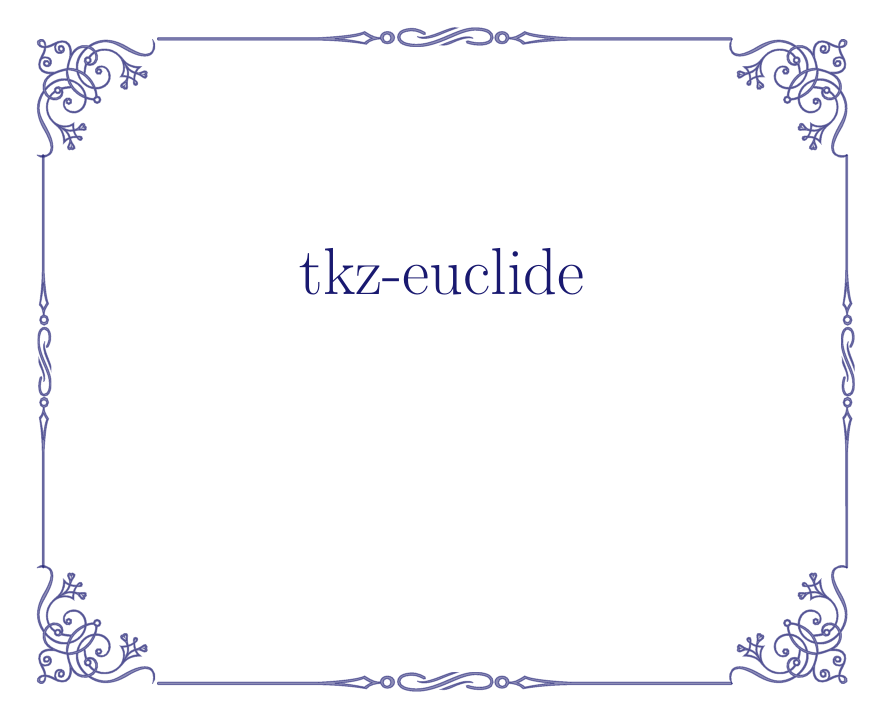
\begin{tikzpicture}
  \coordinate (A) at (0pt,240pt);
  \coordinate (B) at (300pt,240pt);
  \coordinate (C) at (300pt,0pt);
  \coordinate (D) at (0pt,0pt);
  \begin{scope}[opacity=0.5] % for opacity
    \pgfornamentline[color=MidnightBlue]{[xshift=1.65cm,yshift=-1mm]A}{[xshift=-1.58cm,,yshift=-1mm]B}{1}{88}; % AB
    \pgfornamentline[color=MidnightBlue]{[xshift=1.65cm,yshift=1.5mm]D}{[xshift=-1.58cm,yshift=1.5mm]C}{1}{88};
    \pgfornamentline[color=MidnightBlue]{[xshift=2.2mm,yshift=-1.59cm]A}{[xshift=2.2mm,yshift=1.59cm]D}{1}{88};
    \pgfornamentline[color=MidnightBlue]{[xshift=-1.2mm,yshift=-1.59cm]B}{[xshift=-1.2mm,yshift=1.59cm]C}{1}{88};
  \end{scope}
  \node[anchor=north west] at (A) {\pgfornament[color=MidnightBlue,opacity=0.5,width=1.5cm]{61}}; % A
  \node[anchor=north east] at (B) {\pgfornament[color=MidnightBlue,opacity=0.5,width=1.5cm,symmetry=v]{61}};% B
  \node[anchor=south east] at (C) {\pgfornament[color=MidnightBlue,opacity=0.5,width=1.5cm,symmetry=c]{61}}; % C
  \node[anchor=south west] at (D) {\pgfornament[color=MidnightBlue,opacity=0.5,width=1.5cm,symmetry=h]{61}}; % D
  \node[text width=240pt] at (150 pt,120 pt){%
  \begin{center}
    \color{MidnightBlue}
    \fontsize{24}{48}
    \selectfont tkz-euclide\par
                基于\TIKZ 的\par
                欧氏几何绘图宏包
  \end{center}};
\end{tikzpicture}}}
}
\else
\fi
\makeatother
\clearpage
\tkzSetUpColors[background=white,text=darkgray]

\let\rmfamily\ttfamily
\nameoffile{\tkznameofpack}
%\defoffile{\lefthand\
% The \tkzname{\tkznameofpack} is a set of convenient macros for drawing in a
% plane (fundamental two-dimensional object) with a Cartesian coordinate system.
% It  handles the most classic situations in Euclidean Geometry.
% \tkzname{\tkznameofpack} is built on top of PGF and its associated front-end
% \TIKZ\ and is a (La)TeX-friendly drawing package. The aim is to provide a
% high-level user interface  to build graphics  relatively simply. It uses a
% Cartesian coordinate system orthogonal provided by the \tkzimp{tkz-base} package
% as well as tools to define the unique coordinates of points and to manipulate
% them. The idea is to allow you to follow step by step a construction that would
% be done by hand as naturally as possible.\par
% Now the package needs the version 3.0 of \TIKZ. English is  not my native
% language so there  might be some errors.}
\defoffile{\lefthand\
  \tkzname{\tkznameofpack}是一个用于在笛卡尔坐标系中绘制平面图形(点、线、三角形、圆等基本二维
  对象)的尽可能方便使用的宏包,它主要用于绘制经典欧氏几何图形。
  \tkzname{\tkznameofpack}是基于PGF设计的,可以看作是一个\TIKZ{}的前
  端,并且是符合(La)TeX语法的绘图宏包。其目标是提供一个高层的用户
  接口,以通过相对简单语法进行绘图。它使用\tkzname{tkz-base}宏包提供
  的正交笛卡尔坐标系和点的定义及点的操作宏命令为基础进行绘图。该宏包的
  基本思路是尽可能符合欧氏几何中手工绘图的绘图方式。\\
  该宏包需要\TIKZ{}3.0及以上版本支持,另外,由于英语不是母语,该说明文
  档中,可能会存在描述错误。}

\presentation

\vspace*{1cm}
% \lefthand{} Firstly, I would like to thank \textbf{Till Tantau} for the
% beautiful \LaTeX{}  package, namely \href{https://github.com/pgf-tikz/pgf}{\TIKZ}.
\lefthand\ 首先,感谢\textbf{Till Tantau}开发了强大的\TIKZ{}绘图工具\href{https://github.com/pgf-tikz/pgf}{\TIKZ}

\vspace*{12pt}
% \lefthand{} I received much valuable advice, remarks, corrections and examples
% from \tkzimp{Jean-Côme Charpentier}, \tkzimp{Josselin Noirel}, \tkzimp{Manuel Pégourié-Gonnard},
% \tkzimp{Franck Pastor}, \tkzimp{David Arnold}, \tkzimp{Ulrike Fischer}, \tkzimp{Stefan Kottwitz},
% \tkzimp{Christian Tellechea}, \tkzimp{Nicolas Kisselhoff}, \tkzimp{David Arnold},
% \tkzimp{Wolfgang Büchel}, \tkzimp{John Kitzmiller}, \tkzimp{Dimitri Kapetas},
% \tkzimp{Gaétan Marris}, \tkzimp{Mark Wibrow}, \tkzimp{Yves Combe} for his work on a protractor,
% \tkzimp{Paul Gaborit} and \tkzimp{Laurent} for all his corrections, remarks and questions.
\lefthand\ 另外,在宏包开发中,收到了大量有价值的建议、修订、勘误和排版样例。它们主要来自
\tkzimp{Jean-Côme Charpentier}, \tkzimp{Josselin Noirel}, \tkzimp{Manuel Pégourié-Gonnard},
\tkzimp{Franck Pastor}, \tkzimp{David Arnold}, \tkzimp{Ulrike Fischer}, \tkzimp{Stefan Kottwitz},
\tkzimp{Christian Tellechea}, \tkzimp{Nicolas Kisselhoff}, \tkzimp{David Arnold},
\tkzimp{Wolfgang Büchel}, \tkzimp{John Kitzmiller}, \tkzimp{Dimitri Kapetas},
\tkzimp{Gaétan Marris}, \tkzimp{Mark Wibrow}, \tkzimp{Yves Combe}(量角器样例),
\tkzimp{Paul Gaborit} and \tkzimp{Laurent}.

\vspace*{12pt}
% \lefthand{} I would also like to thank Eric Weisstein, creator of MathWorld:
% \href{https://mathworld.wolfram.com/about/author.html}{MathWorld}.
\lefthand\ 感谢MathWorld的创造人Eric Weisstein:
\href{http://mathworld.wolfram.com/about/author.html}{MathWorld}

% \vspace*{12pt}
% \lefthand{} You can find some examples on my site:
% \href{http://altermundus.fr}{altermundus.fr}. \hspace{2cm} under construction!

\vfill

% Please report typos or any other comments to this documentation to:
% \href{mailto:al.ma@mac.com}{\textcolor{blue}{Alain Matthes}}.

如果发现该文档的错误或有其他任何意见和建议,请发信至:\href{mailto:al.ma@mac.com}{\textcolor{blue}{Alain Matthes}}.

如果发现译文的错误或其有他任何意见和建议,请发信至:\href{mailto:nangeng@nwafu.edu.cn}{\textcolor{blue}{耿楠}}.

% This file can be redistributed and/or modified under the terms of the \LaTeX{}
% Project Public License Distributed from \href{http://www.ctan.org/}{CTAN}\
% archives.
可以在\href{http://www.ctan.org/}{CTAN}发布的``LATEX Project Public
License''协议下发布和修改该文档。
\clearpage
\tableofcontents

\clearpage
\newpage

\setlength{\parskip}{1ex plus 0.5ex minus 0.2ex}
\subfileinclude{chap01/TKZdoc-euclide-presentation}
\subfileinclude{chap02/tkzdoc-euclide-installation}
\subfileinclude{chap03/tkzdoc-euclide-news}
\subfileinclude{chap04/tkzdoc-euclide-points}
\subfileinclude{chap05/tkzdoc-euclide-pointsSpc}
\subfileinclude{chap06/tkzdoc-euclide-pointby}
\subfileinclude{chap07/tkzdoc-euclide-pointwith}
\subfileinclude{chap08/tkzdoc-euclide-rnd}
\subfileinclude{chap09/tkzdoc-euclide-lines}
\subfileinclude{chap10/tkzdoc-euclide-triangles}
\subfileinclude{chap11/tkzdoc-euclide-polygons}
\subfileinclude{chap12/tkzdoc-euclide-circles}
\subfileinclude{chap13/tkzdoc-euclide-intersec}
\subfileinclude{chap14/tkzdoc-euclide-angles}
\subfileinclude{chap15/tkzdoc-euclide-sectors}
\subfileinclude{chap16/tkzdoc-euclide-arcs}
\subfileinclude{chap17/tkzdoc-euclide-tools}
\subfileinclude{chap18/tkzdoc-euclide-compass}
\subfileinclude{chap19/tkzdoc-euclide-show}
\subfileinclude{chap20/tkzdoc-euclide-rapporteur}
\subfileinclude{chap21/tkzdoc-euclide-exemples}
\subfileinclude{chap22/tkzdoc-euclide-config}
\subfileinclude{chap23/tkzdoc-euclide-base}
\subfileinclude{chap24/tkzdoc-euclide-faq}

\clearpage\newpage
\small\printindex
\end{document}
